%--------------------------------------------------
%	Chapter 5. GNN Pattern Recognition Algorithm
%--------------------------------------------------

\chapter{Graph Neural Network Pattern Recognition Algorithm}\label{chapter-5}

Once hit-pairs compatible with coming from a particle from a pp collision have been established, they are used to build a graph network. This chapter presents a novel pattern recognition algorithm to prune outlier connections in such a network in order to reconstruct tracks, by utilising GNN architectures. The application of the GNN is focused on the pixel detector, with the aim that the approach will serve as a sophisticated track seeding technique for pixel hits to form preliminary track candidates. If the GNN does not produce a large proportion of fake tracks, such an approach could save significant computational resources. The ultimate aim is to develop a realistic algorithm for track reconstruction that can be deployed in future high-luminosity upgrades of collider detector experiments. This research was presented at the 2022 Connecting the Dots (CTD) conference at the University of Princeton USA and at the dedicated GNN Google DeepMind mini-workshop at UCL in 2023. At the time of writing, this work was under review for publication in the Springer Journal: Computing for Software and Big Science \cite{Lad_2023_gnn}. This chapter is organised as follows; sections \ref{gnn-algorithm-overview} to \ref{gnn-track-extration} present a breakdown of the GNN algorithm and Section \ref{gnn-application-toy-model} illustrates an application on a simple toy MC model.


\section{Algorithm Overview}
\label{gnn-algorithm-overview}

In the context of GNNs, individual hits or clusters of hits are modelled as graph nodes and track segments are modelled as graph edges. Once the graph network is constructed, each edge is modelled as a Gaussian state in order to represent a partial estimate of the track parameters and hence approximate the local track state probability density. Therefore, each node is initialised with a Gaussian mixture of track states, local to its neighbourhood of connections. The GNN-based pattern recognition algorithm is formalised as an iterative mixture reduction problem. This allows the deactivation of incompatible connections (GNN edges termed as outliers), enabling the improvement of track parameter estimates and iterative extraction of track candidates as the network evolves. 

After the initialisation stage, the network evolves iteratively, where an iteration is made up of three main stages illustrated in Figure \ref{fig:flowchart}. 

\begin{figure}[htbp]
    \centering
    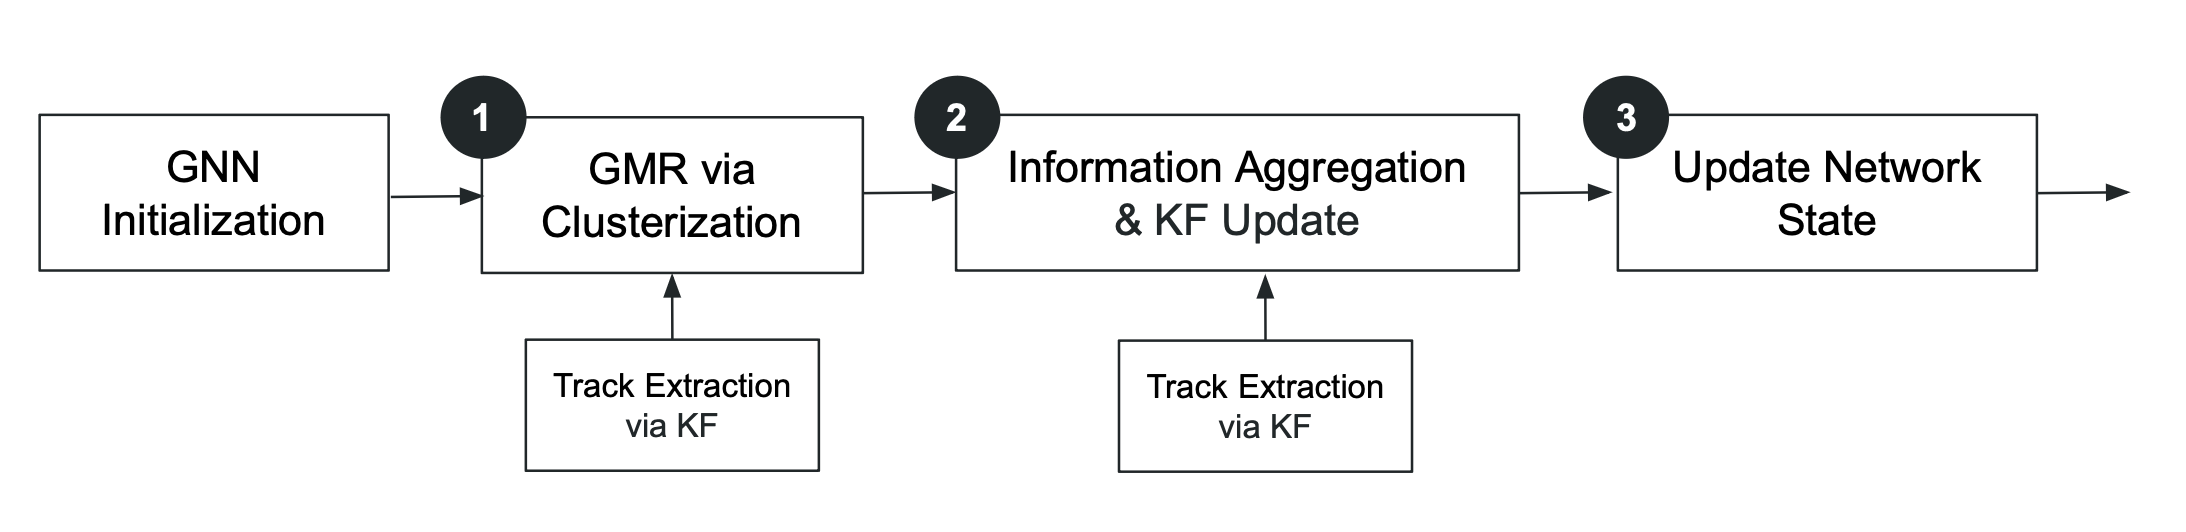
\includegraphics[width=0.98\textwidth]{images/5-gnn-algorithm/gnn-workflow.png}
    \caption{Flow chart illustrating all stages making up an iteration of the GNN-based algorithm. After each stage, a Kalman filter (KF) is applied in order to iteratively extract candidates. After stage three, a further Gaussian Mixture Reduction (GMR) stage would be applied repeating the iterations.}
    \label{fig:flowchart}%
\end{figure}


The first stage applies a Gaussian Mixture Reduction (GMR). This involves a traditional ML approach, whereby compatible Gaussian states are grouped together using clustering techniques and outlier states can be identified. Following this, an Information Aggregation stage is executed, which leverages message passing between adjacent nodes in a neighbourhood. The compatibility of neighbouring states is then assessed via extrapolation, in order to improve local track parameters. The third stage involves updating the network state at each node, with specific connections being deactivated as the network evolves. A graph splitting algorithm is also applied directly after the first two stages, in order to identify good track candidates, and if discovered they are extracted. 

Unlike traditional methodologies whereby MLPs are employed for deep learning strategies \cite{Caillou:28155782}, the proposed GNN leverages simplified KFs embedded in the network which are used for two main purposes. Firstly, the KF is embedded directly into the algorithm and used as a mechanism for information propagation during the second stage, such that the precision of track parameters can be iteratively improved. Secondly, the KF is used to apply a track fit for the extraction of compatible track candidates. This allows the algorithm to efficiently exploit a priori knowledge about charged particle dynamics as the network evolves.

The excitation and inhibition rules of individual edge connections are designed to facilitate the “simple-to-complex” approach for “hits-to-tracks” association, such that the network starts with low hit density regions of an event and gradually progresses towards more complex areas. As the network evolves, the uncertainty in local track parameters decreases until there are no more track candidates that fulfil the criteria for a good track. This is the end state of the network where isolated nodes, track fragments and unresolved ambiguities will remain.



\section{Graph Network Initialization}
\label{gnn-network-initialization}

The graph network is implemented using the Python library \texttt{NetworkX} \cite{SciPyProceedings_11}. Hits from a particle event are represented as nodes and predicted hit-pairs as edge connections. Typically, track detection inefficiencies are random such that they cannot be learned. One approach to mitigating this is to allow edge connections to be built spanning up to two detector layers apart, ensuring random cases when a track is not detected in the intermediate layer. See Chapter \ref{chapter-4} for further details on the hit-pair predictor used to form edge connections. Following this, a common graph theory technique known as Connected Component Analysis (CCA), is applied using a built-in function of NetworkX \cite{networkx}. CCA detects connected regions in data structures and splits the network into smaller, more manageable, graphs referred to as \textit{subgraphs}. 

The general approach is formalised as follows. Each pairwise connection between node $i$ and neighbour node $j$ forms a Gaussian state, $X_{ij}$, representing the local track parameter estimate. Each edge has an associated prior probability $p_{ij}$ and edge weight $w_{ij}$. The prior probability of nodes $i$ and $j$ belonging to the same track is determined, assuming a track can produce at most one hit per detector layer. $w_{ij}$ is a mixture weight for the compatibility of the Gaussian state transmitted from node $i$ to neighbour node $j$, and represents the strength of the connection. The weights $w_{ij}$ are initialised uniformly and are dependent on the number of neighbours local to a node. The parameters $w_{ij}$ and $p_{ij}$ are updated as the network evolves. Note that $w_{ij}$ are not to be confused with the traditional weights associated to features within neural networks. 

For a given node $i$ and neighbour nodes $j$, a Gaussian mixture $g_i(X)$ is formed from weighted components, $\Phi_{ij}$, representing a partial estimate of track state parameters, where the general form of $g_i(X)$ is given by Eq \eqref{eqn:gaussian-mixture},


\begin{equation}
g_i(X) = \sum_{j} w_{ij}\Phi_{ij}(X, X_{ij}, C_{ij})
\label{eqn:gaussian-mixture}
\end{equation}

where $C_{ij}$ are track state covariances. All edges act as bidirectional conduits, such that message passing can occur in both directions. All edges are initialised as \textit{active}, allowing the propagation of state information between its node-pair, whereas \textit{deactivated} or \textit{non-active} edges do not allow state information to be propagated. 

%Figure \ref{fig:network-initial} illustrates a node and its neighbourhood.

% \begin{figure}[htbp]%
%     \centering
%     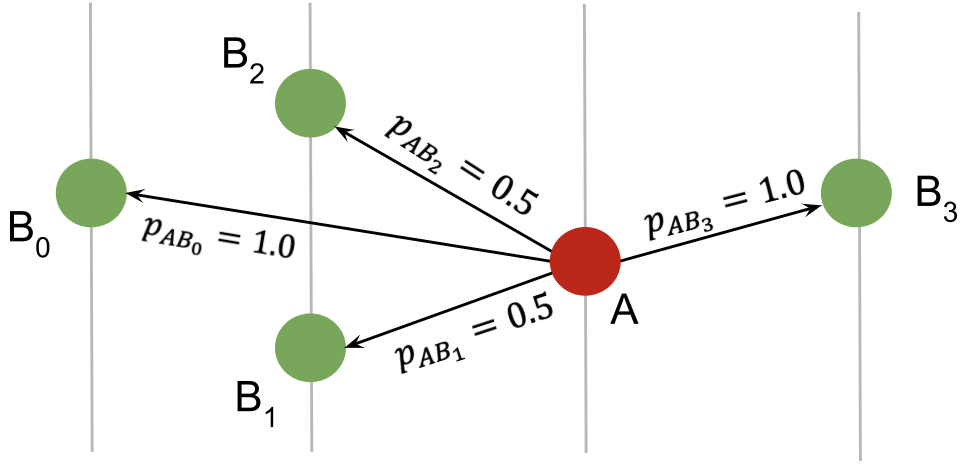
\includegraphics[width=8.8cm]{images/5-gnn-algorithm/network-initialisation.png}%
%     \caption{Prior probabilities associated to network edges of node A's local neighbourhood. Neighbours $B_j$ are located on separate detector layers shown by vertical lines. The unidirectional edges indicate the direction of propagation of state information and priors. These entities will differ from nodes $B_j$ distributing messages to their corresponding neighbourhoods.}%
%     \label{fig:network-initial}%
%\end{figure}




\section{Gaussian Mixture Reduction}
\label{section-GMR}

For nodes with a high multiplicity of edge connections, the number of potential track states can quickly rise. To make inferences within a reasonable amount of processing time, GMR is used to prevent the number of components from exploding. One computationally efficient algorithm for GMR is clustering. A high multiplicity Gaussian mixture can be approximated by one with lower multiplicity, using the traditional k-means clustering \cite{kmeans}. At each node, similar track states are grouped together forming a reduced mixture and their corresponding edges remain active, as illustrated in Figure \ref{fig:GMR-example}. By default, clustering is only applied to nodes with more than two active edge connections.


\begin{figure}[htbp!] 
    \centering
    \subfloat[]{%
        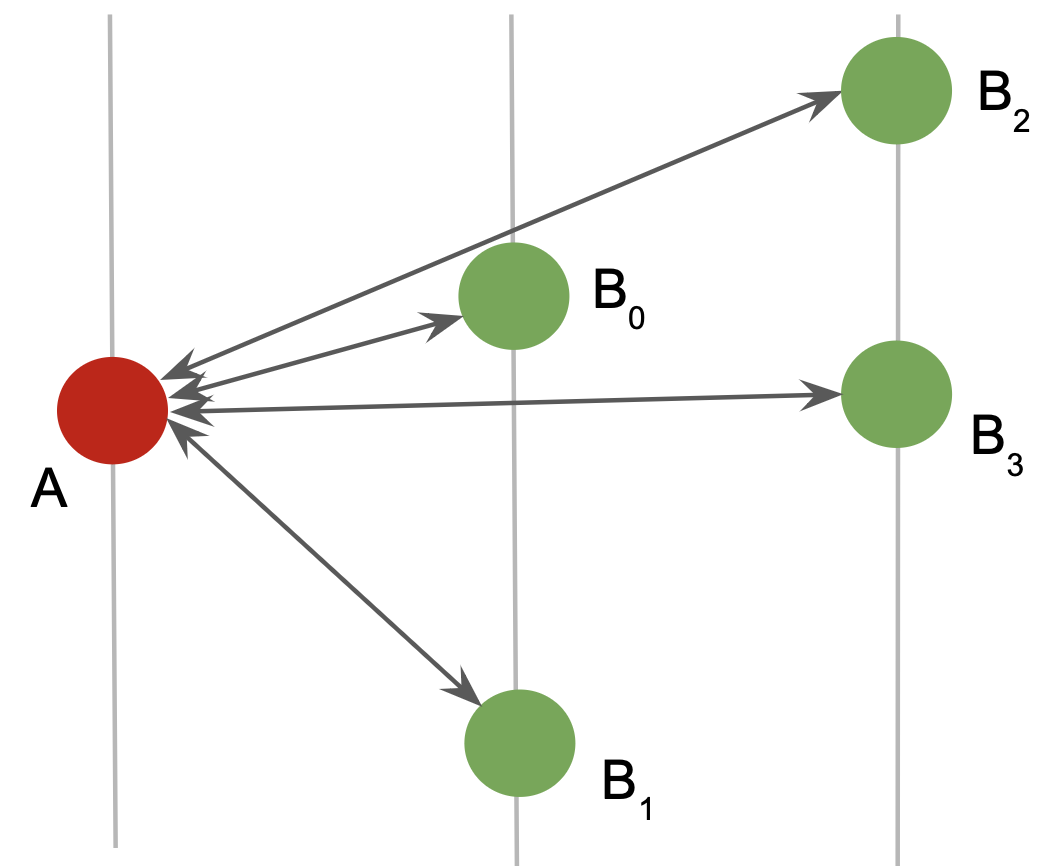
\includegraphics[width=0.42\linewidth]{images/5-gnn-algorithm/GMR-1.png}%
        \label{fig:GMR-1}%
        }%
    \hfill%
    \subfloat[]{%
        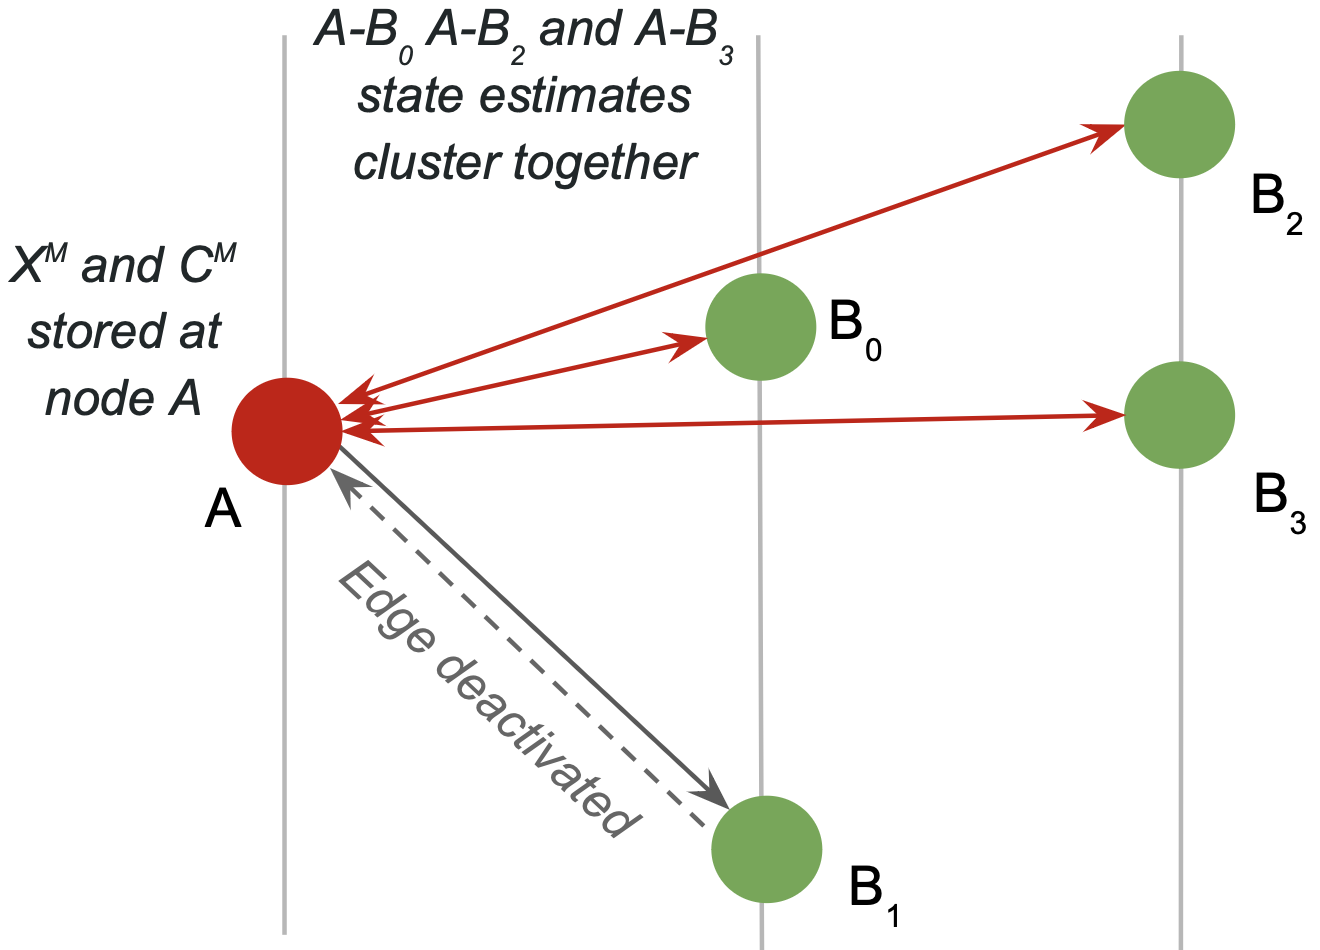
\includegraphics[width=0.57\linewidth]{images/5-gnn-algorithm/GMR-2.png}%
        \label{fig:GMR-2}%
        }%
    \caption{Illustration of GMR via clustering applied to graph networks. Independent detector layers are represented by the vertical lines.}
    \label{fig:GMR-example}
\end{figure}


Figure \ref{fig:GMR-1} shows node $A$ and its local neighbourhood $B_j$ with bidirectional edge connections. Figure \ref{fig:GMR-2} shows the expected result of GMR applied to node $A$. If clustering is successful, a merged track state estimate, $X^M$, is formed from states $X_{AB_0}$, $X_{AB_2}$, $X_{AB_3}$ clustered together and the corresponding merged state covariance, $C^M$, is formed from $C_{AB_0}$, $C_{AB_2}$, $C_{AB_3}$. Outlier states are simultaneously identified and their edges are deactivated. The incoming $B_1 - A$ edge has been deactivated (represented as a dotted line), as any incoming state information from neighbour $B_1$ is deemed incompatible at node $A$.

The merged state estimate $X^{M}$ and merged state covariance $C^{M}$ are computed using the inverse-variance weighting \cite{inverse-variance-weighting} given by Eq \eqref{eqn:inverse-variance-weighting}, where $G_{ij}$ = $C_{ij}^{-1}$.

\begin{equation}
    X^{M} = C^{M} \sum_{j} G_{ij} X_{ij},  \quad  C^{M} = \left( \sum_{j} G_{ij} \right) ^{-1}
    \label{eqn:inverse-variance-weighting}
\end{equation}

The k-means clustering is implemented using the general case of $k=1$, to model the Gaussian mixture at each node as a single track with outlier connections. For the case where a node is located in close proximity to an intersection between two tracks, two or more clusters can be expected. In such a case, the mixture reduction process is declared impossible. This part of the network remains dormant until competing edges are deactivated through information propagation from other parts of the network and the mixture becomes more unimodal. The current implementation is a limitation of k-means clustering, as the number of clusters to form at each node must be predetermined, which is a non-trivial task. An alternative procedure would include the use of DBSCAN for clustering, as no prior knowledge of the number of clusters is required as this information is determined by the clustering algorithm and would be useful in regions with intersecting tracks. However, when considering the computational complexity of such approaches, the k-means algorithm scales linearly, $O(n)$, with the number of edges $n$, compared to DBSCAN which scales non-linearly, $O(n^2)$. The work presented in this thesis is limited to the general case of k=1 case, where the extension k $>$ 1 would require further exploration. 


\subsection{The Kullback-Leibler Divergence}
In order to establish whether clustering can occur for a given node, a distance measure is used as a threshold. The Kullback-Leibler (KL) divergence \cite{KL, FRUHWIRTH19971}, $d_{KL}$, is a measure of the statistical distance between two Gaussian probability distributions and is used in the k-means algorithm to determine if track states can be grouped into a cluster. The $d_{KL}$ between $X_{ij}$ and $X_{ik}$ is given by Eq \eqref{eqn:kullback-leibler}.

\begin{equation}
    d_{KL} = tr[(C_{ij} - C_{ik})(G_{ij} - G_{ik})] + (X_{ij} - X_{ik})^{T}(G_{ij} + G_{ik})(X_{ij} - X_{ik})
    \label{eqn:kullback-leibler}
\end{equation}

The optimal $d_{KL}$ threshold will differ for each node depending on its local neighbourhood. For example, consider a node with a high empirical variance of edge orientation in its neighbour connections, $\sigma_{e}^{2}$. The corresponding $d_{KL}$ threshold will be larger in comparison to a node with a small $\sigma_{e}^{2}$, where neighbour connections are more closely orientated. To determine the optimal $d_{KL}$ threshold between pairwise $X_{ij}$ for a given node, a SVM classifier was trained against truth information using a MC simulation. See Section \ref{chapter-6-kl-threshold} for further details on the implementation.

In principal, a physical distance can also serve as an alternative measure within the clustering algorithm, such as the Euclidean distance between two neighbour nodes. However, the choice of the KL divergence is preferred over the Euclidean distance, as it is a general measure of the difference between two probability distributions. Given the underlying assumption that each edge is a partial estimate of the track parameters with corresponding mean and covariance, both of these entities are taken into account by the KL divergence, and hence reflects its statistical meaning. The KL divergence seeks to measure the correlation between variables, as it incorporates the covariance between the two measured states. In general, a state can be defined by parameters other than spatial coordinates, i.e. parameters encoded into some latent representation, therefore it is also important to consider the covariance.



\section{Information Aggregation}

\subsection{Message Passing}
Neural message passing in graph networks effectively captures the dependencies and interactions among nodes, by providing a framework to exchange information with their neighbour nodes and aggregate that information to update their own representations. Both structural information of the graph and the features associated with each node are captured.

The message passing mechanism is leveraged in the GNN algorithm in order to improve the precision of track state parameters on a local and global scale. During the previous stage (Section \ref{section-GMR}), reduced Gaussian mixtures were formed for nodes where clustering was successful. For a given node $i$, $X^M$ and $C^M$ are propagated to all neighbours $j$ which have active $i \rightarrow j$ connections. If clustering was unsuccessful for a particular node, this part of the network remains dormant until a merged state is received via message passing during later stages of the algorithm. Track state information can be propagated in both directions along active network edges. This ensures that the compatibility of received states can be validated and assessed against each node's local neighbourhood.


\subsection{Validation}
Once state information has been propagated to neighbours, the parameter estimation begins with a linear projection of the incoming track state onto the subspace of measurements. As illustrated in Figure \ref{fig:extrapolation}, for a given node $i$, each incoming $X^M$ is projected via a measurement matrix $H$, which relates the incoming track state to the measurement values. See Section \ref{gnn-application-toy-model} for implementation of matrix $H$. In order to validate if the connection between nodes $i$ and $j$ is compatible, the Mahalanobis distance \cite{mahalanobis-distance}, $\Delta \chi^{2}_{ij}$, is calculated using the residual between the projected state, $HX$, and the measurement at the neighbour node, $m$. The threshold $d_{\chi^{2}}$ is a tuned hyperparameter and represents the maximum $\Delta \chi^{2}_{ij}$ acceptable for an incoming track state. If $\Delta \chi^{2}_{ij} \leq d_{\chi^{2}}$, the connection is deemed compatible and the state can be extrapolated via a KF. If $\Delta \chi^{2}_{ij} > d_{\chi^{2}}$ then the connection is deemed incompatible and the corresponding edge is deactivated.

% \begin{figure}[htbp]
\begin{figure}[H]
        \centering
        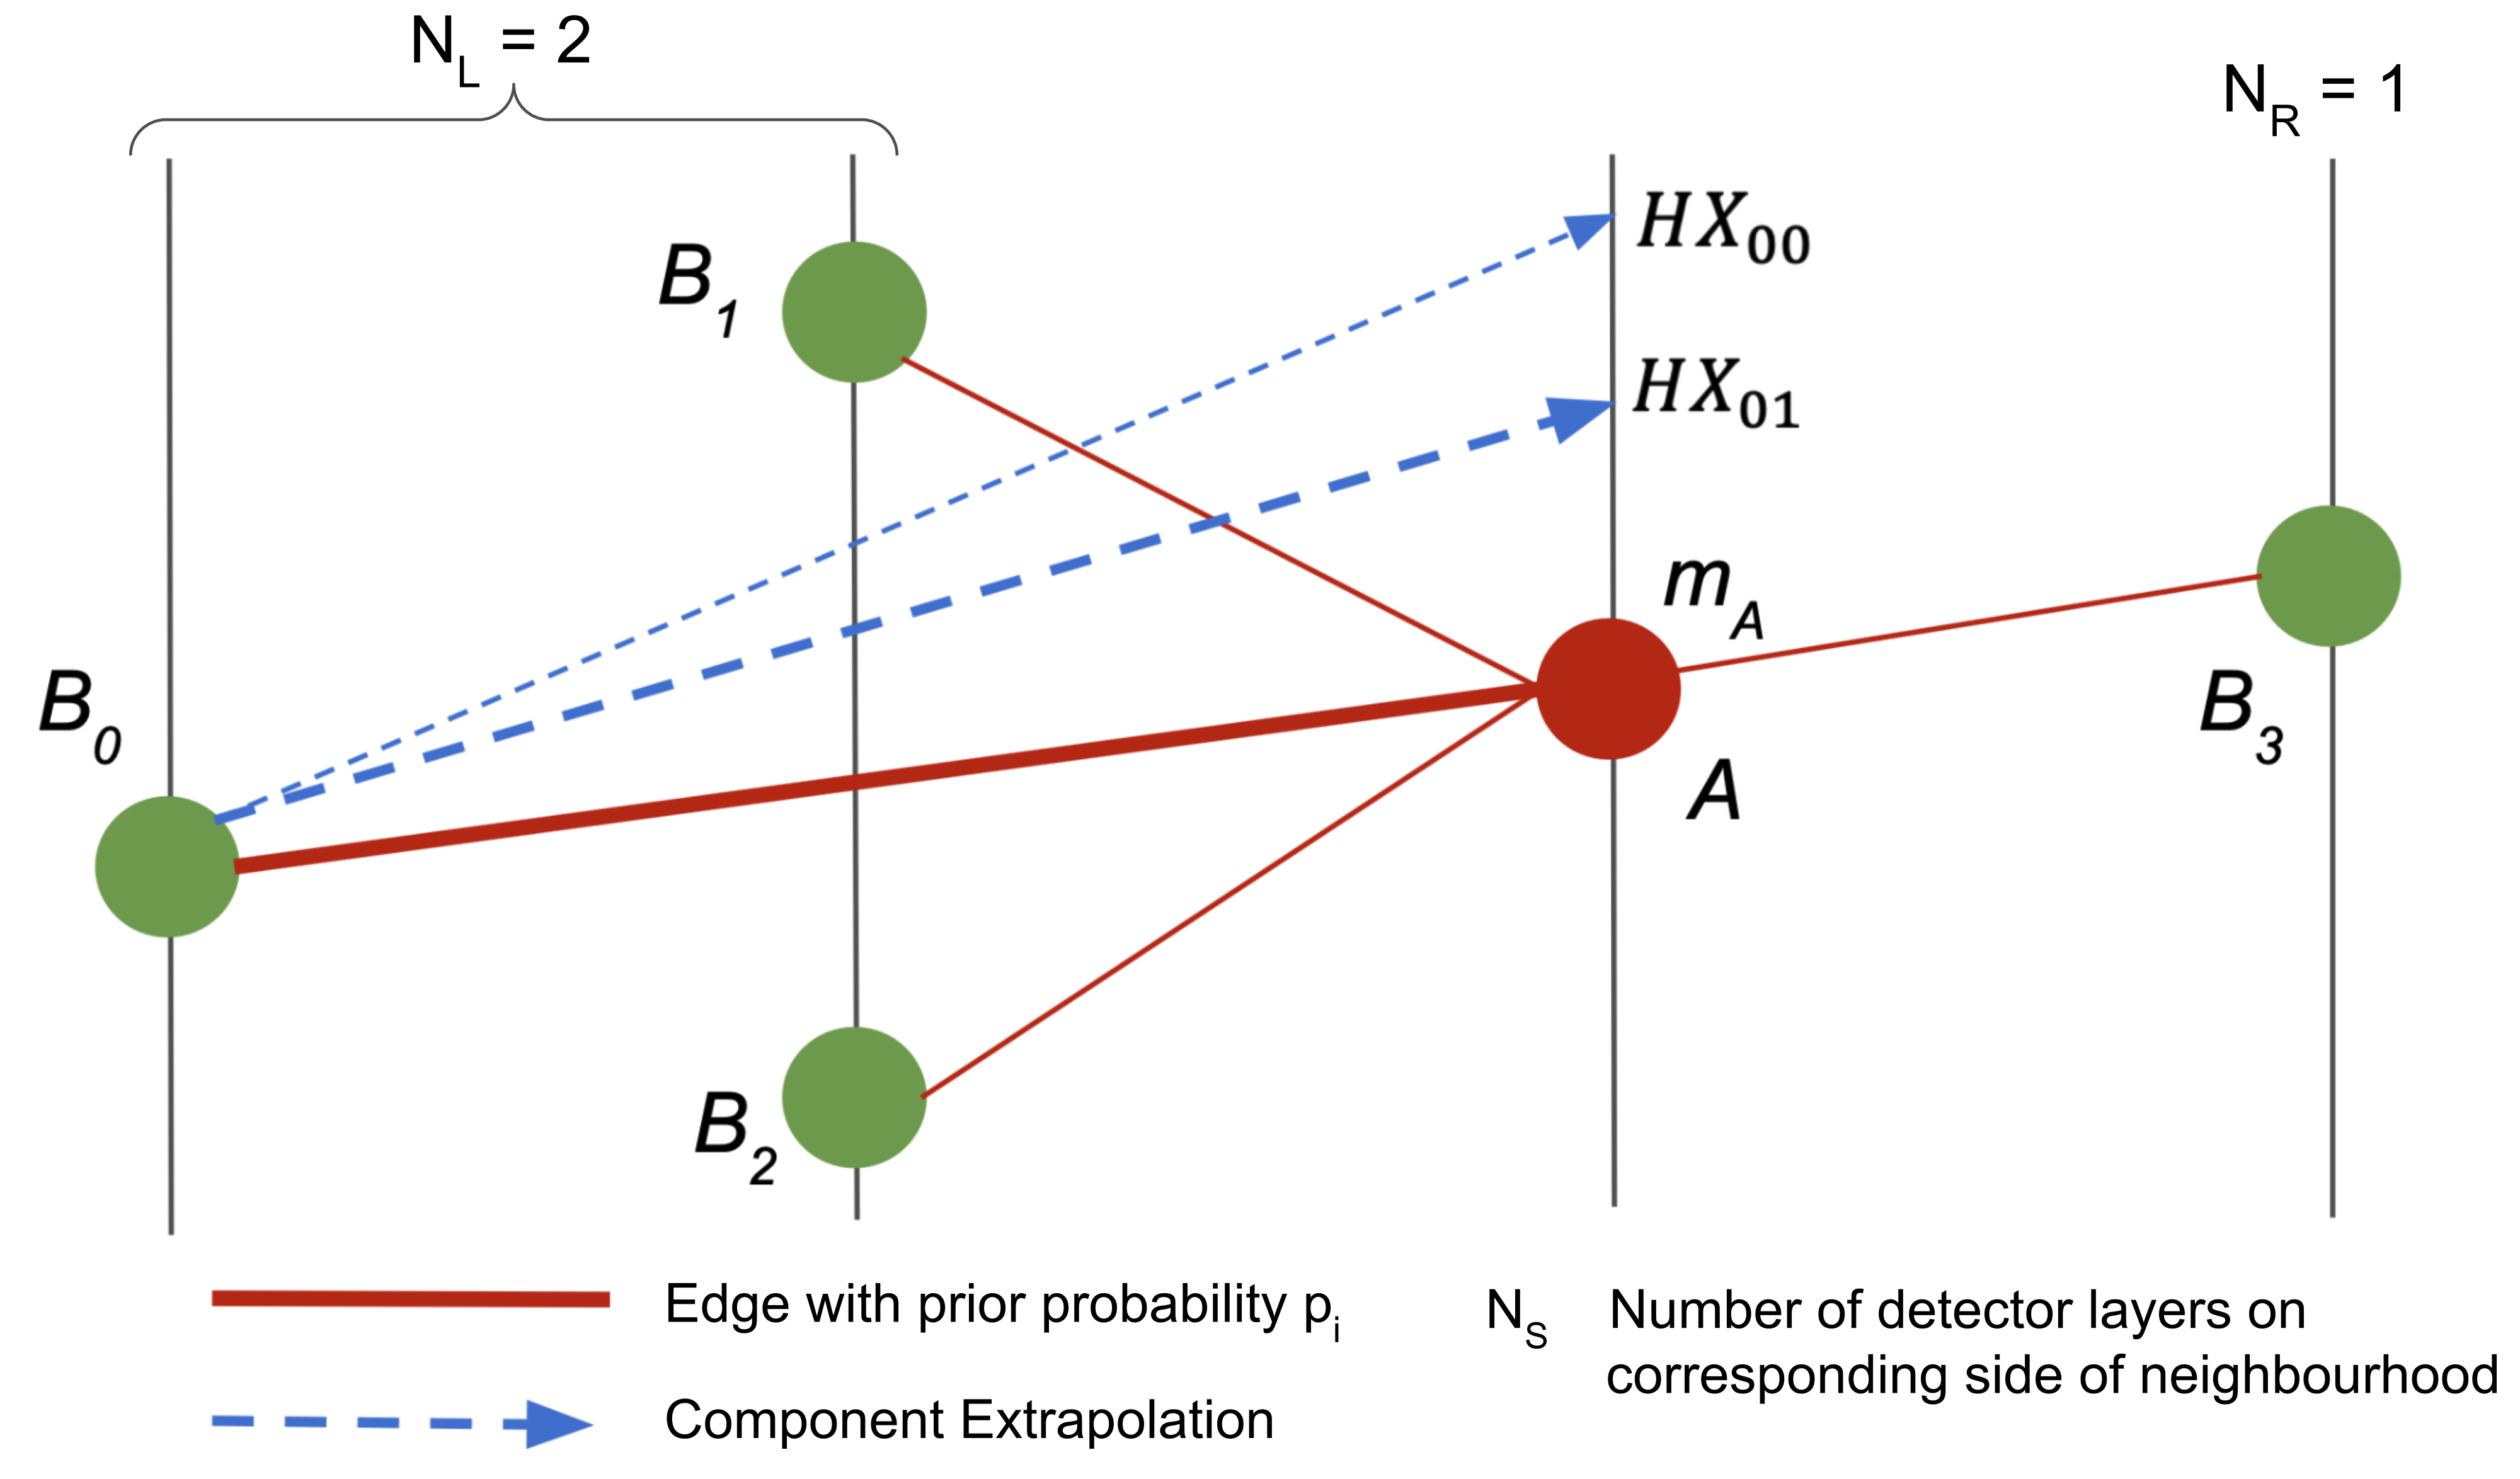
\includegraphics[width=0.95\textwidth]{images/5-gnn-algorithm/gnn-extrapolation.png}
        \caption{Illustration of track state estimates $X_{00}$ and $X_{01}$ being projected from node $B_0$ to node $A$ via a measurement matrix $H$ into the subspace of measurements. $m_A$ is the measurement at node $A$. The corresponding residual between $m_A$ and the projected incoming state from $B_0$ is used to compute the Mahalanobis distance $\Delta \chi^{2}$ to determine if the incoming state is compatible with $m_A$. $N_L$ indicates the number of detector layers on the left side of node $A$'s local neighbourhood, and $N_R$ indicates the number of detector layers on the right side, where the detector layers are represented by the vertical lines.}
        \label{fig:extrapolation}%
\end{figure}


\subsection{KF Update and Extrapolation}
\label{chapter-5-kf-extrapolation}

For compatible incoming states where $\Delta \chi^{2}_{ij} \leq d_{\chi^{2}}$, the KF update is applied in order to compute the extrapolated track state estimate, $\tilde{X}_{ij}$, and the corresponding extrapolated covariance matrix, $\widetilde{C}_{ij}$. The KF is implemented via the Python library \texttt{Filterpy} \cite{filterpy}. $\tilde{X}_{ij}$ and $\widetilde{C}_{ij}$ are given by Eqs. \eqref{eqn:extrapolation},

\begin{equation}
\tilde{X}_{ij} = F_{ij} X_{ij}^{M}, \qquad \tilde{C}_{ij} = F_{ij} \biggl( \sum C_{ij}^{M} + Q_{ij} \biggl) F^{T}_{ij}
\label{eqn:extrapolation}
\end{equation}

where $F_{ij}$ is the state transition Jacobian from node $i$ to node $j$, and $Q$ is the process noise matrix. See Section \ref{gnn-application-toy-model} for implementation of the KF update, including the transition Jacobian $F$ and process noise $Q$. 






\section{Updating Network State}
\label{gnn-updating-network-state}

As the network evolves and specific connections are deactivated, the local track parameter estimates change at each node. Therefore, the corresponding edge weights, $w_{ij}$, should reflect this for the strength of each connection, hence $w_{ij}$ are updated. Given the underlying assumption that each edge is modelled as a Gaussian probability density function, with corresponding mean and covariance, a Gaussian measurement likelihood is used to update $w_{ij}$. For the connection between nodes $i$ and $j$, the updated edge weights $\widetilde{w}_{ij}$ are computed using the normalised Gaussian measurement likelihood given by Eq \eqref{eqn:likelihood}, 

\begin{equation}
\beta_{ij} = (2 \pi \lvert S_{ij} \rvert )^{-1/2}  e^{-\Delta \chi^{2}_{ij} / 2}
\label{eqn:likelihood}
\end{equation}

where $S_{ij}$ is the joint measurement covariance matrix and $\Delta \chi^{2}_{ij}$ is the Mahalanobis distance between the projected state the measurement. The updated edge weights $\widetilde{w}_{ij}$ are given by Eq \eqref{eqn:weights}, 

\begin{equation}
\widetilde{w}_{ij} = \frac{1}{N_S} \frac{w_{ij}\beta_{ij} p_{ij}}{\sum_{k}w_{ik}\beta_{ik}}
\label{eqn:weights}
\end{equation}


where $p_{ij}$ are the prior probabilities as described in Section \ref{gnn-network-initialization}. The denominator $\sum_{k}w_{ik}\beta_{ik}$ is the summation of the product of weights and likelihoods in the neighbourhood of node $i$. The weights $\widetilde{w}_{ij}$ are divided by the number of detector layers on either side of its neighbourhood, $N_S$, in order to account for the probability that a track passing through node $i$ was detected at layer $L$. If $\widetilde{w}_{ij} < 0.1$, the corresponding edge connection is automatically deactivated as the likelihood of compatibility of this incoming track state is extremely low. This forms part of the mechanism for edge activation and deactivation. The Gaussian mixture $g_i(X)$ at each node is then composed of updated components, given by Eq \eqref{eqn:updated-gaussian-mixture}.

\begin{equation}
g_i(X) = \sum_{j} \widetilde{w}_{ij}\Phi_{ij}(X, \widetilde{X}_{ij}, \widetilde{C}_{ij})
\label{eqn:updated-gaussian-mixture}
\end{equation}

Following this update, the algorithm iterations repeat. A further GMR would follow, clustering on $\widetilde{X}_{ij}$. This allows further ambiguities to be resolved and the precision of track state parameters to be increased at each additional stage.






\section{Graph Splitting and Track Extraction}
\label{gnn-track-extration}

The design of the GNN-based framework is such that it is possible to iteratively discover track candidates after each stage. As shown in Figure \ref{fig:flowchart}, a track extraction algorithm is executed after the GMR and Information Aggregation stages.

Initially, the graph network must be split into smaller components, taking into account only edges which remain active. A CCA is applied to the network by using the NetworkX built-in function \texttt{weakly\_connected\_components}. This ensures that smaller, more manageable subgraphs are separated from the main network.

The criteria that a subgraph must satisfy in order to be considered for track extraction are as follows. Subgraphs must contain a minimum number of four nodes within the volume of interest. There must exist only one node per detector layer, so that there are no intersecting tracks or holes within the track candidate. 

If the above criteria are met, a KF is then applied in order to perform a final track fit. As opposed to applying the KF on one track segment between two nodes, similar to the method used in Section \ref{chapter-5-kf-extrapolation} for state extrapolation, the KF for track fitting considers the whole chain of track segments. Here, the filter iteratively predicts and updates track state parameters as it receives measurements from each subsequent node in the subgraph. The KF is initialised with a filter state estimate, $\hat{x}$, a filter state covariance, $\hat{P}$, state transition Jacobian, $\hat{F}$, measurement function, $\hat{H}$, measurement noise $\hat{R}$ and process noise, $\hat{Q}$.

In order to assess the quality of the track fit the p-value is computed from the $\chi^2$ statistic. The p-value obtained must be greater than 0.01. Subgraphs that fulfill all conditions are defined as good track candidates and are extracted from the network, such that their corresponding nodes and edges are removed. Subgraphs that do not meet the above criteria for track extraction, remain in the graph network for further processing.





\section{Application on a Simple MC Model}
\label{gnn-application-toy-model}

A linear 2-dimensional MC model was used to simulate seven truth tracks in the $x$-$y$ plane, each with ten hits as shown in Figure \ref{fig:ground-truth}. 

\begin{figure}[htbp]
    \centering
    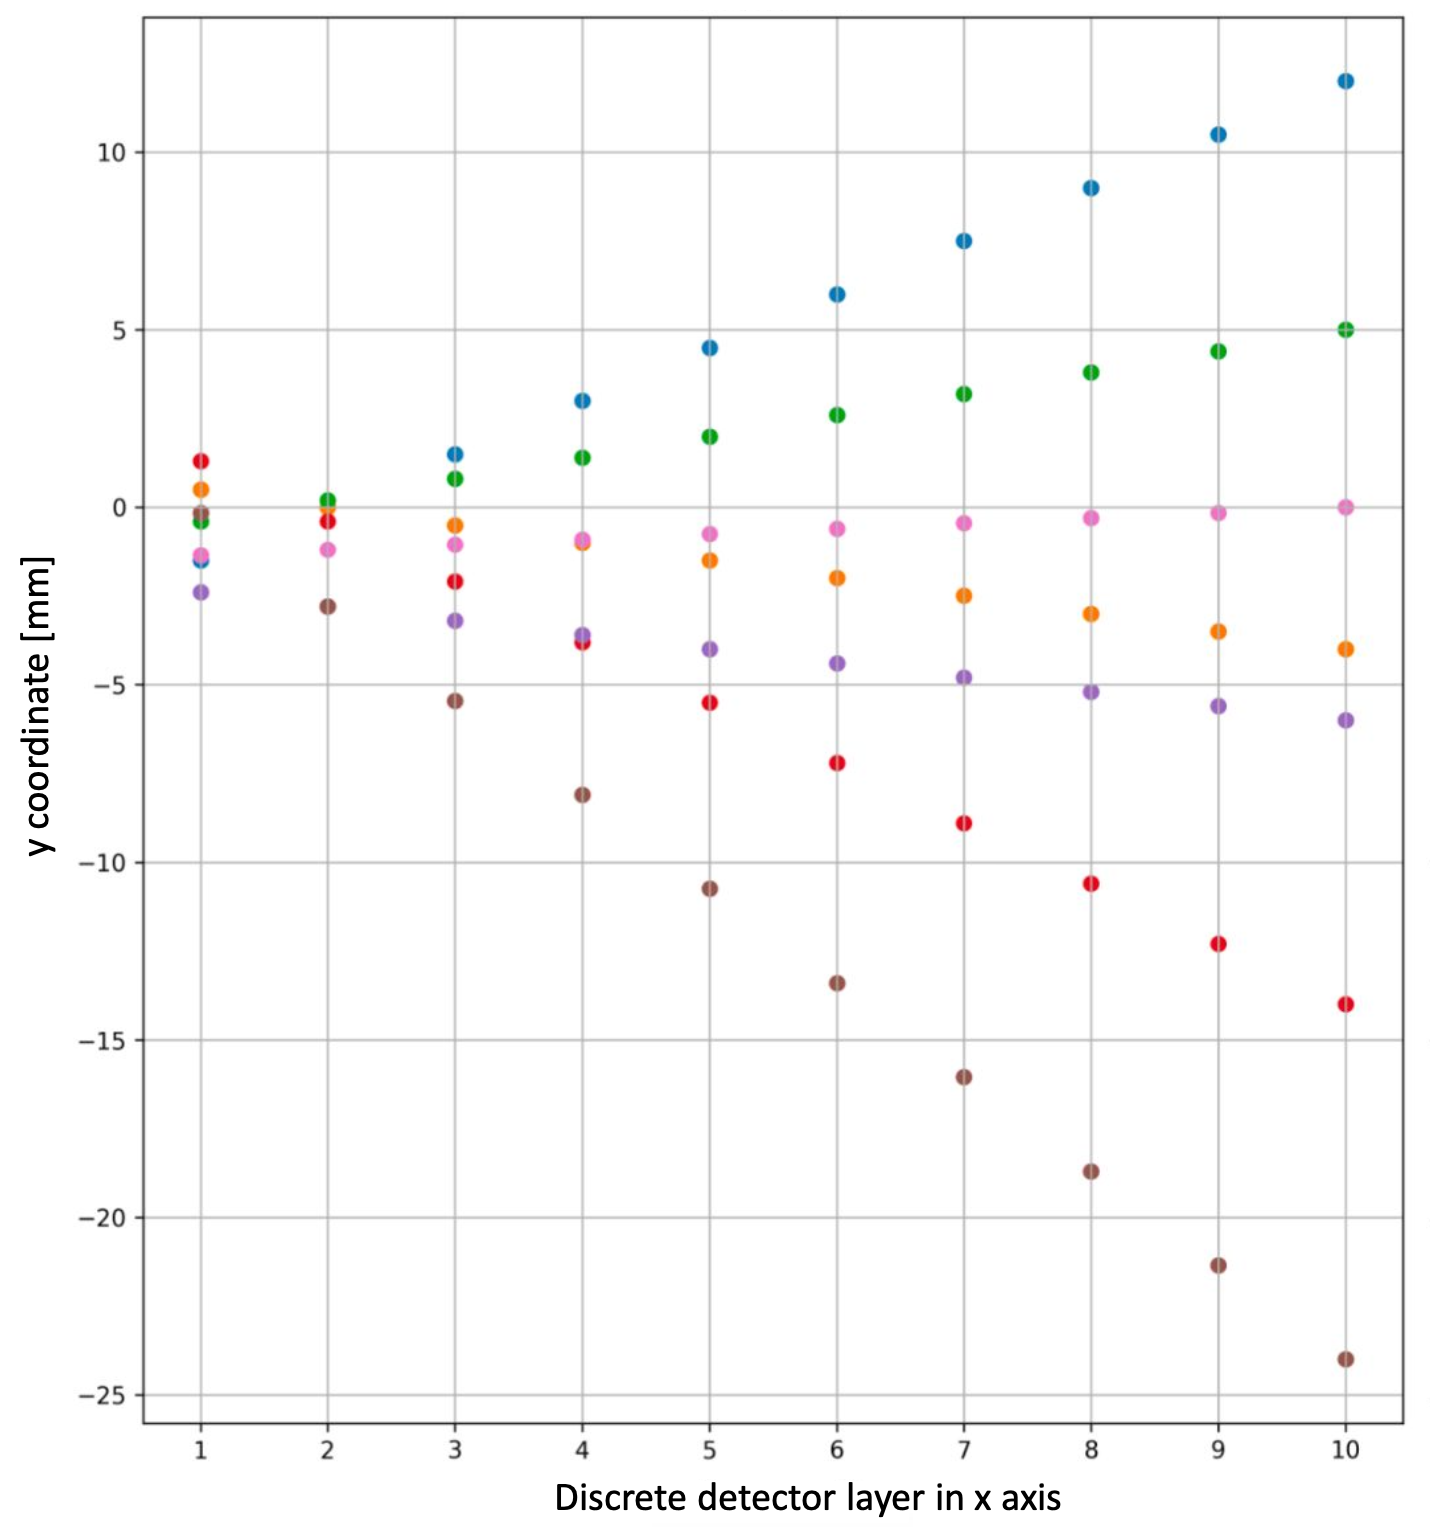
\includegraphics[width=0.78\textwidth]{images/5-gnn-algorithm/ground-truth.png}
    \caption{Simulation of seven truth tracks.}
    \label{fig:ground-truth}%
\end{figure}

Random Gaussian noise was added to the $y$-coordinate in order to simulate measurement error. The track position measurements, $m$, are given by Eq \eqref{eqn:mc-toy-measurement-model}

\begin{equation}
m = y + \sigma_0 \delta
\label{eqn:mc-toy-measurement-model}
\end{equation}

where $y$ is the unobserved track positions, $\sigma_0$ is the standard deviation in the measurement of the $x$-$y$ plane and is initialised to 100 $\mu$m, and $\delta$ is a Gaussian random variable with zero mean and variance of one.

The graph network was formed using a many-to-one mapping of hits-to-nodes, where hits in close proximity within each layer were merged into one node. The threshold for the merging was determined using the distance distribution between hits located in the same layer. To build edge connections and reduce all possible combinatorics between node pairs, a simple edge-predictor method was devised. The predictor is loosely based on the ideas discussed in Chapter \ref{chapter-4} and uses the track inclination of neighbour nodes. If the inclination of a neighbour node spanning up to two layers apart is within a particular range, this edge is deemed compatible and a connection is established. 

The node degree (the number of edges associated to each node) and the empirical variance of edge orientation in its neighbour connections, $\sigma_{e}^{2}$, provide indications of neighbourhood complexity. For example, nodes which have a high multiplicity of connections indicate areas where there are significant outliers to resolve, and vice versa for nodes with low degree. This feature is illustrated by Figure \ref{fig:heat-map}, which shows a heat map labelled by node degree. High degree nodes are referred to as ``hot'' (white-yellow) and low degree nodes are referred to as ``cold'' (orange-red).


% \begin{figure}[htbp]
\begin{figure}[H]
    \centering
    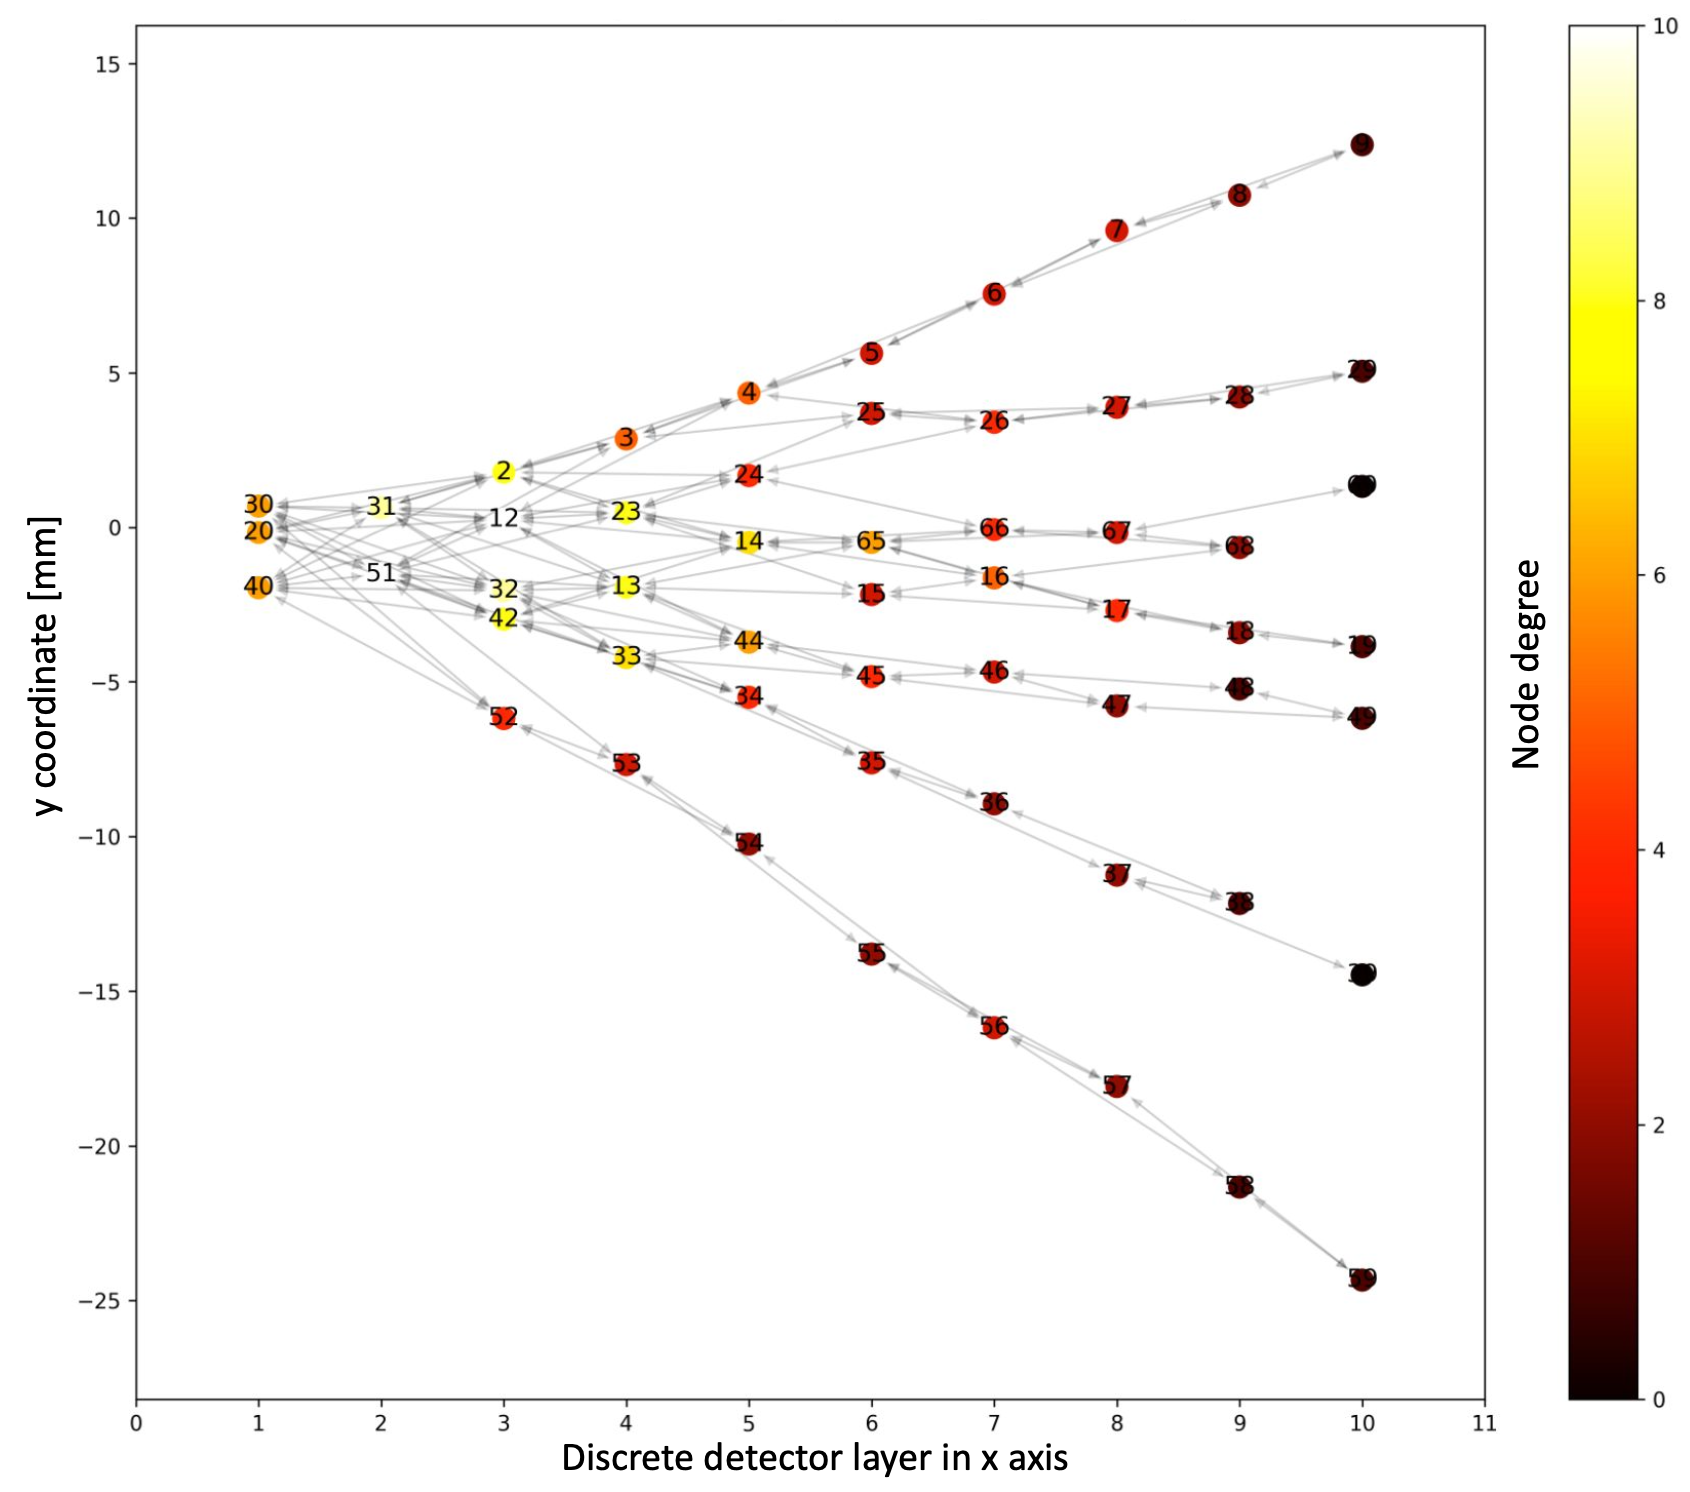
\includegraphics[width=0.99\textwidth]{images/5-gnn-algorithm/heatmap-network.png}
    \caption{Conversion of simulated hits in Figure \ref{fig:ground-truth} to a graph network, plotted as a node-degree heat map using the model in Eq \eqref{eqn:mc-toy-measurement-model}. Edge connections are formed using a pair predictor. The heat map represents node degree, where ``hot'' nodes (white-yellow) contain many edge connections, whereas ``cold'' nodes (orange-red) contain fewer edge connections.}
    \label{fig:heat-map}%
\end{figure}


\subsubsection{Graph Network Initialization}

The network is initialised with track state estimates, $X_{ij}$, given by Eq \eqref{eqn:track-state-estimate} and MC truth information at each node. Each connection is modelled as a straight line, where $X_{ij}$ comprises the $y$-measurement at node $i$, given by $m_i$, and the track inclination to its neighbour node $j$, given by $\tau_{ij} = (m_i - m_j) / (x_i - x_j)$, so that

\begin{equation}
X_{ij} = \begin{bmatrix} m_i \\ \tau_{ij} \end{bmatrix}
\label{eqn:track-state-estimate}
\end{equation}


The joint measurement covariance matrix, $S$, is stated in Eq. \eqref{eqn:track-state-estimate-2}, where $\sigma_0$ = 100 $\mu$m. Negligible uncertainty is assumed in the $x$-measurement due to the low thickness of pixel sensors. The state covariance, $C_{ij}$, is derived using the standard linear algebra approach, where $C_{ij} = GSG^T$, where matrix $G$ is the Jacobian which relates the measurements to the state vector, $X_{ij}$, using a linear extrapolation, where $dx = x_i - x_j$.  

\begin{equation}
S = \begin{bmatrix} \sigma_0^{2} & 0 \\ 0 & \sigma_0^{2} \end{bmatrix}  \quad G = \begin{bmatrix} 1 & 0 \\ dx^{-1} & -dx^{-1}  \end{bmatrix}
\label{eqn:track-state-estimate-2}
\end{equation}


\subsubsection{Implementation of Track State Extrapolation}

During Stage 1: GMR, $X^{M}$ and $C^{M}$ are computed using Eq \eqref{eqn:inverse-variance-weighting}. During Stage 2: Information Aggregation, $X^M$ is projected into the subspace of measurements using the measurement vector $H = [1 \quad 0]$. The residual, $r_{ij}$, between the projection, $HX^M$, and the measurement at each node is calculated using Eq \eqref{eqn:residual}

\begin{equation}
r_{ij} = m_i - HX_{ij}^M
\label{eqn:residual}
\end{equation}

The covariance of the residual, $V_{ij}$, is given by Eq. \eqref{eqn:covariance-of-residual}

\begin{equation}
{V}_{ij} = H \widetilde{C}_{ij} H^{T} + \sigma_{0}^{2}
\label{eqn:covariance-of-residual}
\end{equation}

where the extrapolated covariance, $\widetilde{C}_{ij}$, is calculated using Eq \eqref{eqn:extrapolation} with process noise, $Q$, defined as the zero matrix. The corresponding Mahalanobis distance is given by Eq \eqref{eqn:mahalanobis-distance}, and the distribution can be seen in Figure \ref{fig:mahalanobis-threshold-toy-model}.

\begin{equation}
\Delta \chi_{ij}^{2} = r_{ij}^{T} {V}_{ij}^{-1} r_{ij}
\label{eqn:mahalanobis-distance}
\end{equation}


% \begin{figure}[htbp]
\begin{figure}[H]
    \centering
    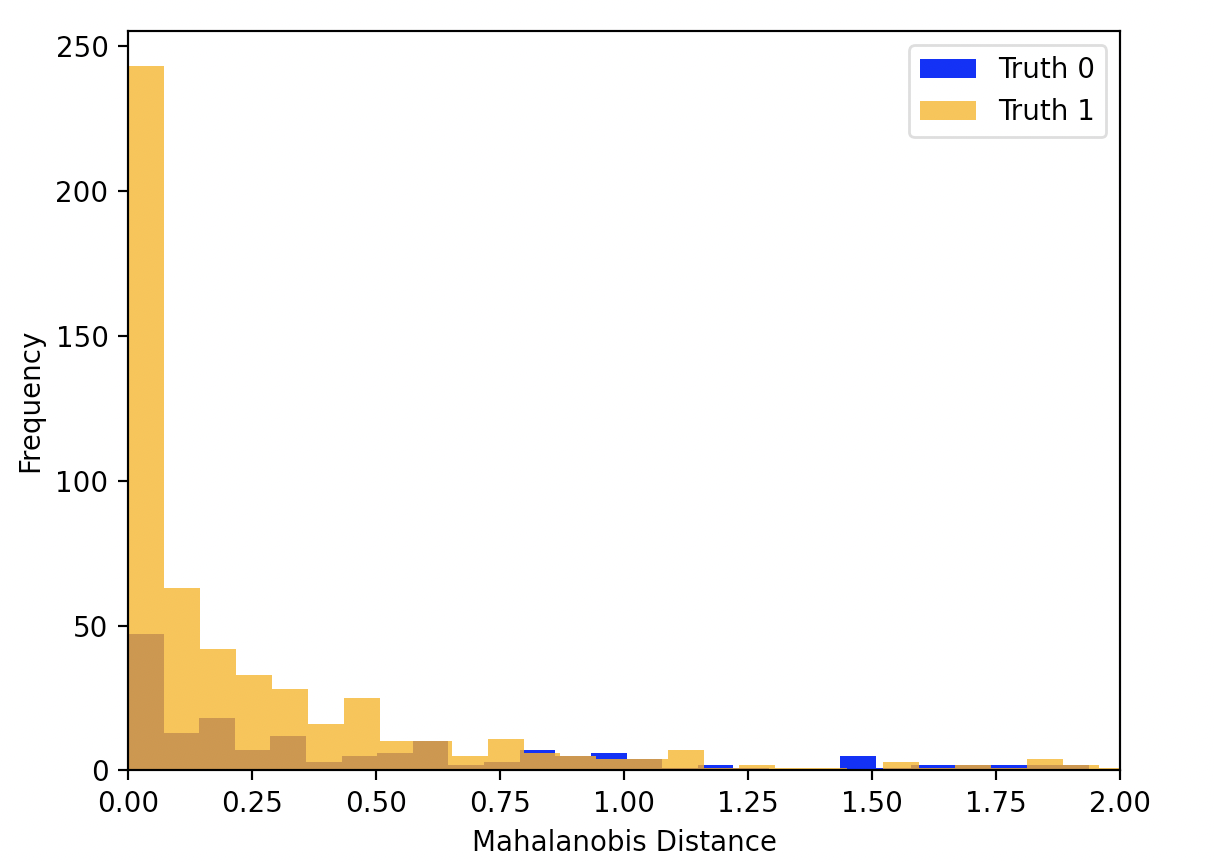
\includegraphics[width=0.96\textwidth]{images/5-gnn-algorithm/mahalanobis-threshold-toy-model-2.png}
    \caption{Mahalanobis distance, $\Delta \chi^{2}$, computed between the projected state and the measurement at each node, during state extrapolation for the GNN algorithm applied to a simple toy MC model. Truth 1 shows the distribution where the truth particle originating from the extrapolated state and the truth particle originating from the measurement are the same, and truth 0 otherwise.}
    \label{fig:mahalanobis-threshold-toy-model}%
\end{figure}



Using Figure \ref{fig:mahalanobis-threshold-toy-model}, a distance of 1.0 is selected as a threshold for accepting extrapolated states, as this provides 95\% efficiency on selecting the truth 1 class. If $\Delta \chi_{ij}^{2} < 1.0$, then $X^M$ is extrapolated to its neighbour node using the KF update. The extrapolated state, $\widetilde{X}_{ij}$, is calculated by the KF using Eq \eqref{eqn:extrapolation}, defined as the linear extrapolation from node $j$ to node $i$. This is described by $m_i = m_j + \tau_j dx$ and $\tau_i = \tau_j$. Therefore, the derived Jacobian, $\hat{F}$, for the KF is given by Eq \eqref{eqn:mc-model-F}.

% Jacobian F is derived by differentation of m_i and t_i equations with respect to initial parameters m_j and t_j

\begin{equation}
\hat{F} = \begin{bmatrix} 1 & dx \\ 0 & 1 \end{bmatrix}
\label{eqn:mc-model-F}
\end{equation}



\subsubsection{Implementation of KF for Track Extraction}

For a set of $n$ nodes representing a track candidate, the sequential set of measurements are $\{m_{(n-1)}, ..., m_1, m_0 \}$, where $m_{(n-1)}$ is the measurement of the node with the largest radius. The KF for track extraction is initialised with the following two-dimensional filter state estimate, $\hat{x}$, given by Eq \eqref{eqn:kf-toy-model-x-init}.

\begin{equation}
\hat{x} = \begin{bmatrix} m_{(n-1)} \\ \tau_{(n-1)} \end{bmatrix}
\label{eqn:kf-toy-model-x-init}
\end{equation}

where the track position measurement, $m_{(n-1)}$, is known and the track inclination, $\tau_{(n-1)}$, is initialized to zero as track inclination information is unknown at the start of the filter. The filter covariance matrix, $\hat{P}$, is initialised using Eq \eqref{eqn:mc-model-P-init-covariance}

\begin{equation}
\hat{P} = \begin{bmatrix} \sigma_0^{2} & 0 \\ 0 & \sigma_{\tau}^2 \end{bmatrix}
\label{eqn:mc-model-P-init-covariance}
\end{equation}

where $\sigma_{\tau}^2$ is the variance in the track inclination, $\tau$, and is initialized to $10^3$. The measurement error in the KF, $\hat{R}$, is attributed to the error due to the measurement of the $x$-$y$ plane and is initialised to $\sigma_{0}$ = 100 $\mu$m. The transition Jacobian in the KF uses the linear model and is given by Eq \eqref{eqn:mc-model-F}. The measurement vector is given by $\hat{H} = [1 \quad 0]$ and the process noise matrix is set to $\hat{Q} = 0$.



\subsubsection{Results}

Figure \ref{fig:example-application-1} shows an example of the GNN algorithm applied to the toy model in Figure \ref{fig:heat-map}. Figure \ref{fig:mc-example-1} displays the graph network where an initial CCA has been applied. Three smaller subgraphs have been identified as shown by separate colours. Nodes with $\sigma_e^2 > 0.8$ are not shown as clustering was not possible. The subsequent extracted track candidates are shown in Figure \ref{fig:mc-example-2}, where seven distinct tracks are observed. A precision of 60\% was achieved on identifying correct outlier connections with respect to the MC truth during stage 1. This simulation shows 100\% efficiency of track reconstruction with respect to MC truth, as all seven truth tracks were extracted in two stages. 

Figure \ref{fig:example-application-2} shows another simulation of the MC toy track model with application of the GNN algorithm. The application of CCA yields two distinct subgraphs shown in Figure \ref{fig:mc-example-3} by two separate colours. The subsequent extracted track candidates are shown in Figure \ref{fig:mc-example-4}, where six distinct tracks can be observed. A precision of 65\% was achieved on identifying correct outlier connections with respect to the MC truth during stage 1. A fast convergence was achieved in extracting six out of seven track candidates after the first stage of the algorithm. Remaining networks were propagated to further stages, however no further track candidates were extracted. Similarly, nodes with $\sigma_e^2 > 0.8$ are not shown here, as clustering was not possible. This suggests that $\sigma_{e}^{2}$ is an important discriminating feature when clustering track state estimates. 

Within this simple example, the GNN-based algorithm was not continued beyond stage 2. The main aim was to illustrate that the iterative methodology of the GNN framework is successful in identifying outlier edge connections as the graph network evolves, and allows track candidates to become easily identifiable. The purpose here was not to reconstruct the entire track candidate in all pixel layers of this model (nodes with $\sigma_e^2 > 0.8$). This task would require further analysis and optimisation of hyperparameters. At the time of writing, investigation of the application of the GNN-based algorithm on a realistic detector setup with much greater hit multiplicity was prioritised. Proper tuning of hyperparameters is done for the TrackML detector model, discussed further in Chapter \ref{chapter-6}. 


%\begin{center}
\begin{figure}[htbp]%
    \centering
    \subfloat[\centering Simulated graph network post CCA]{{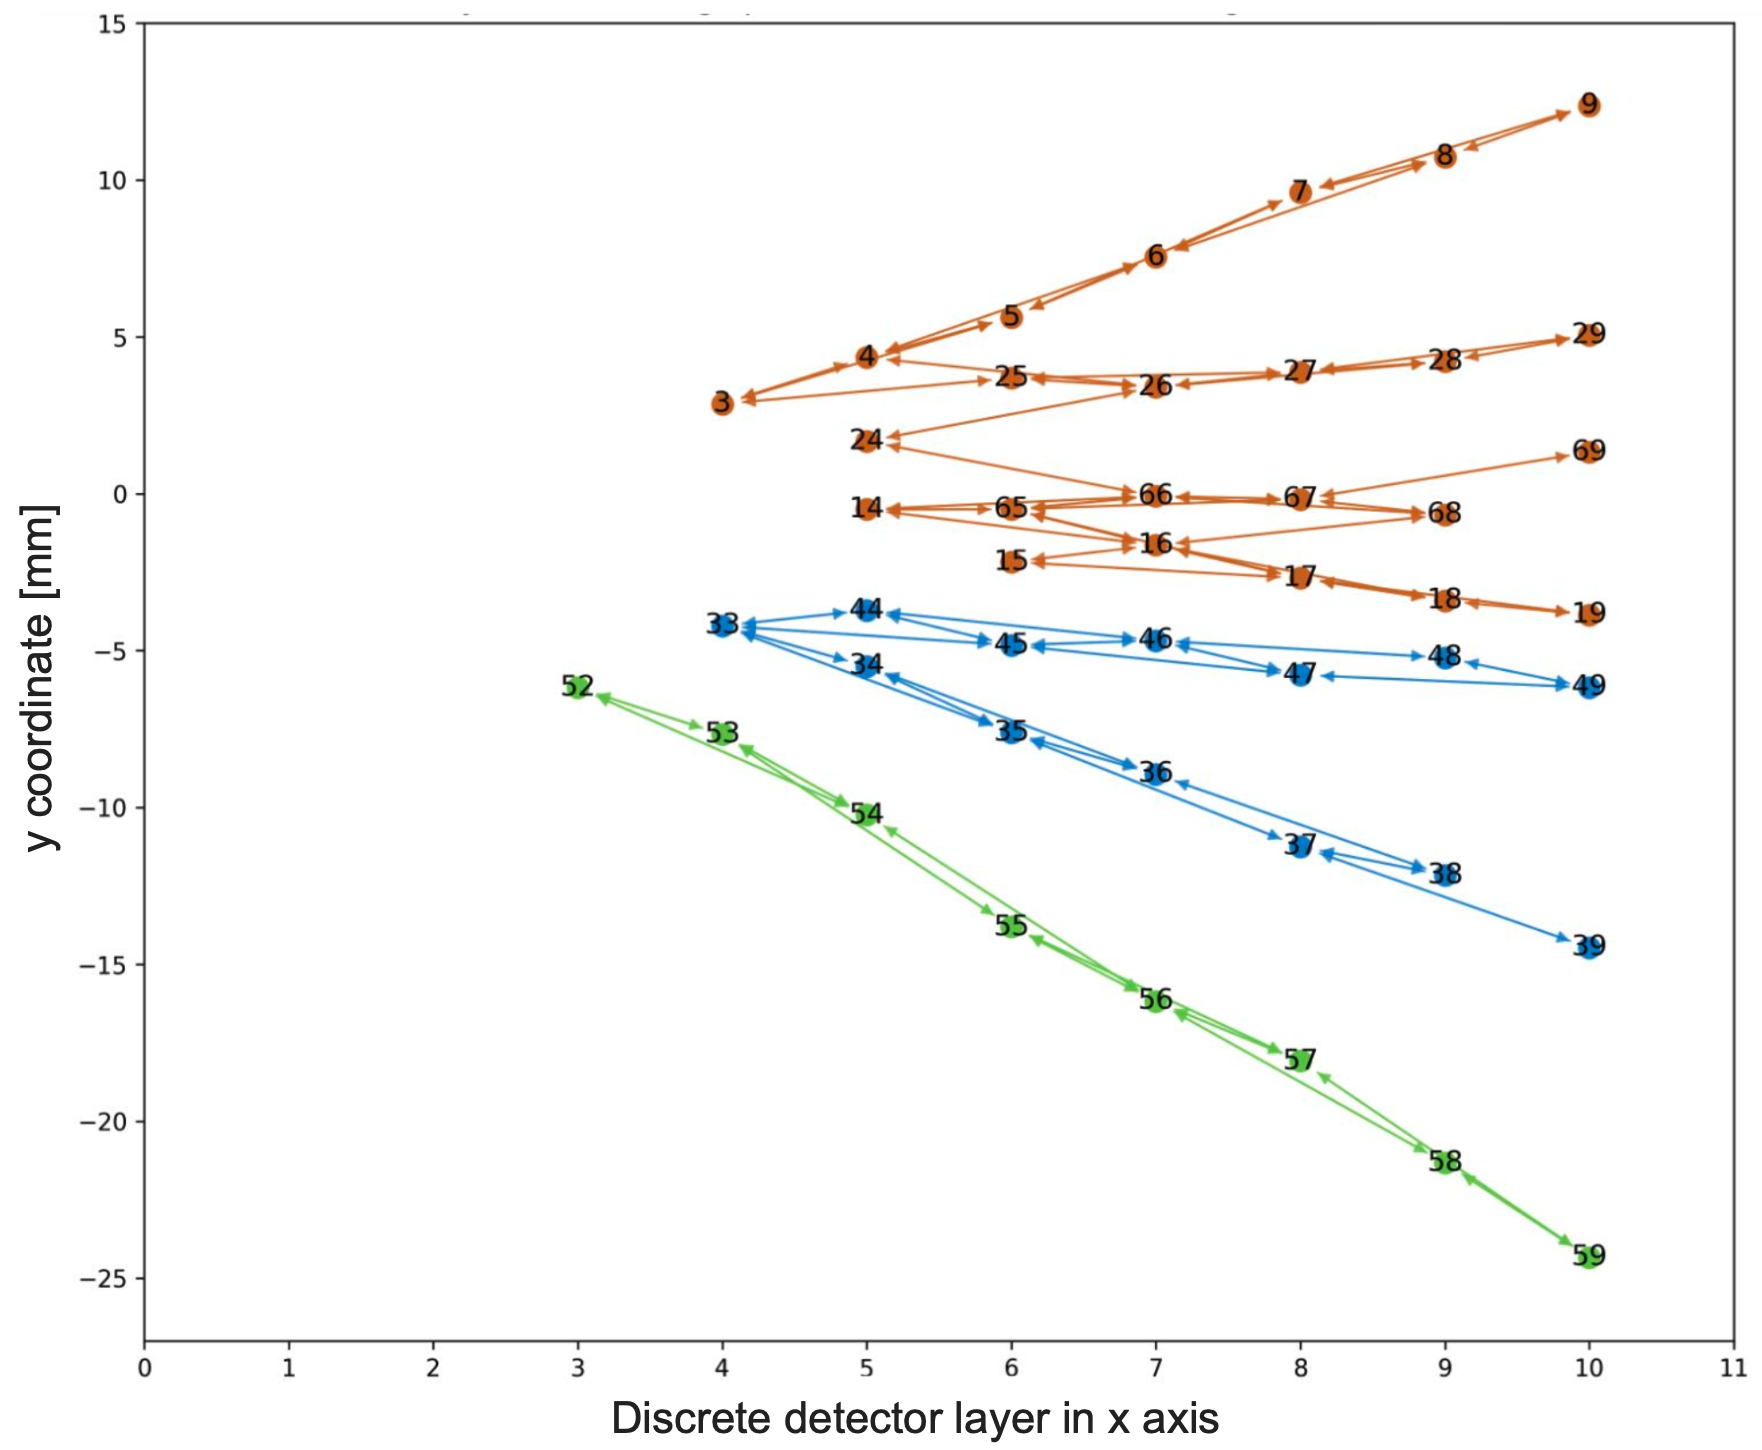
\includegraphics[width=11.8cm]{images/5-gnn-algorithm/mc-example-1a.png} } \label{fig:mc-example-1}}%
    \hfill
    %\qquad
    \subfloat[\centering Extracted track candidates at each stage of the GNN algorithm]{{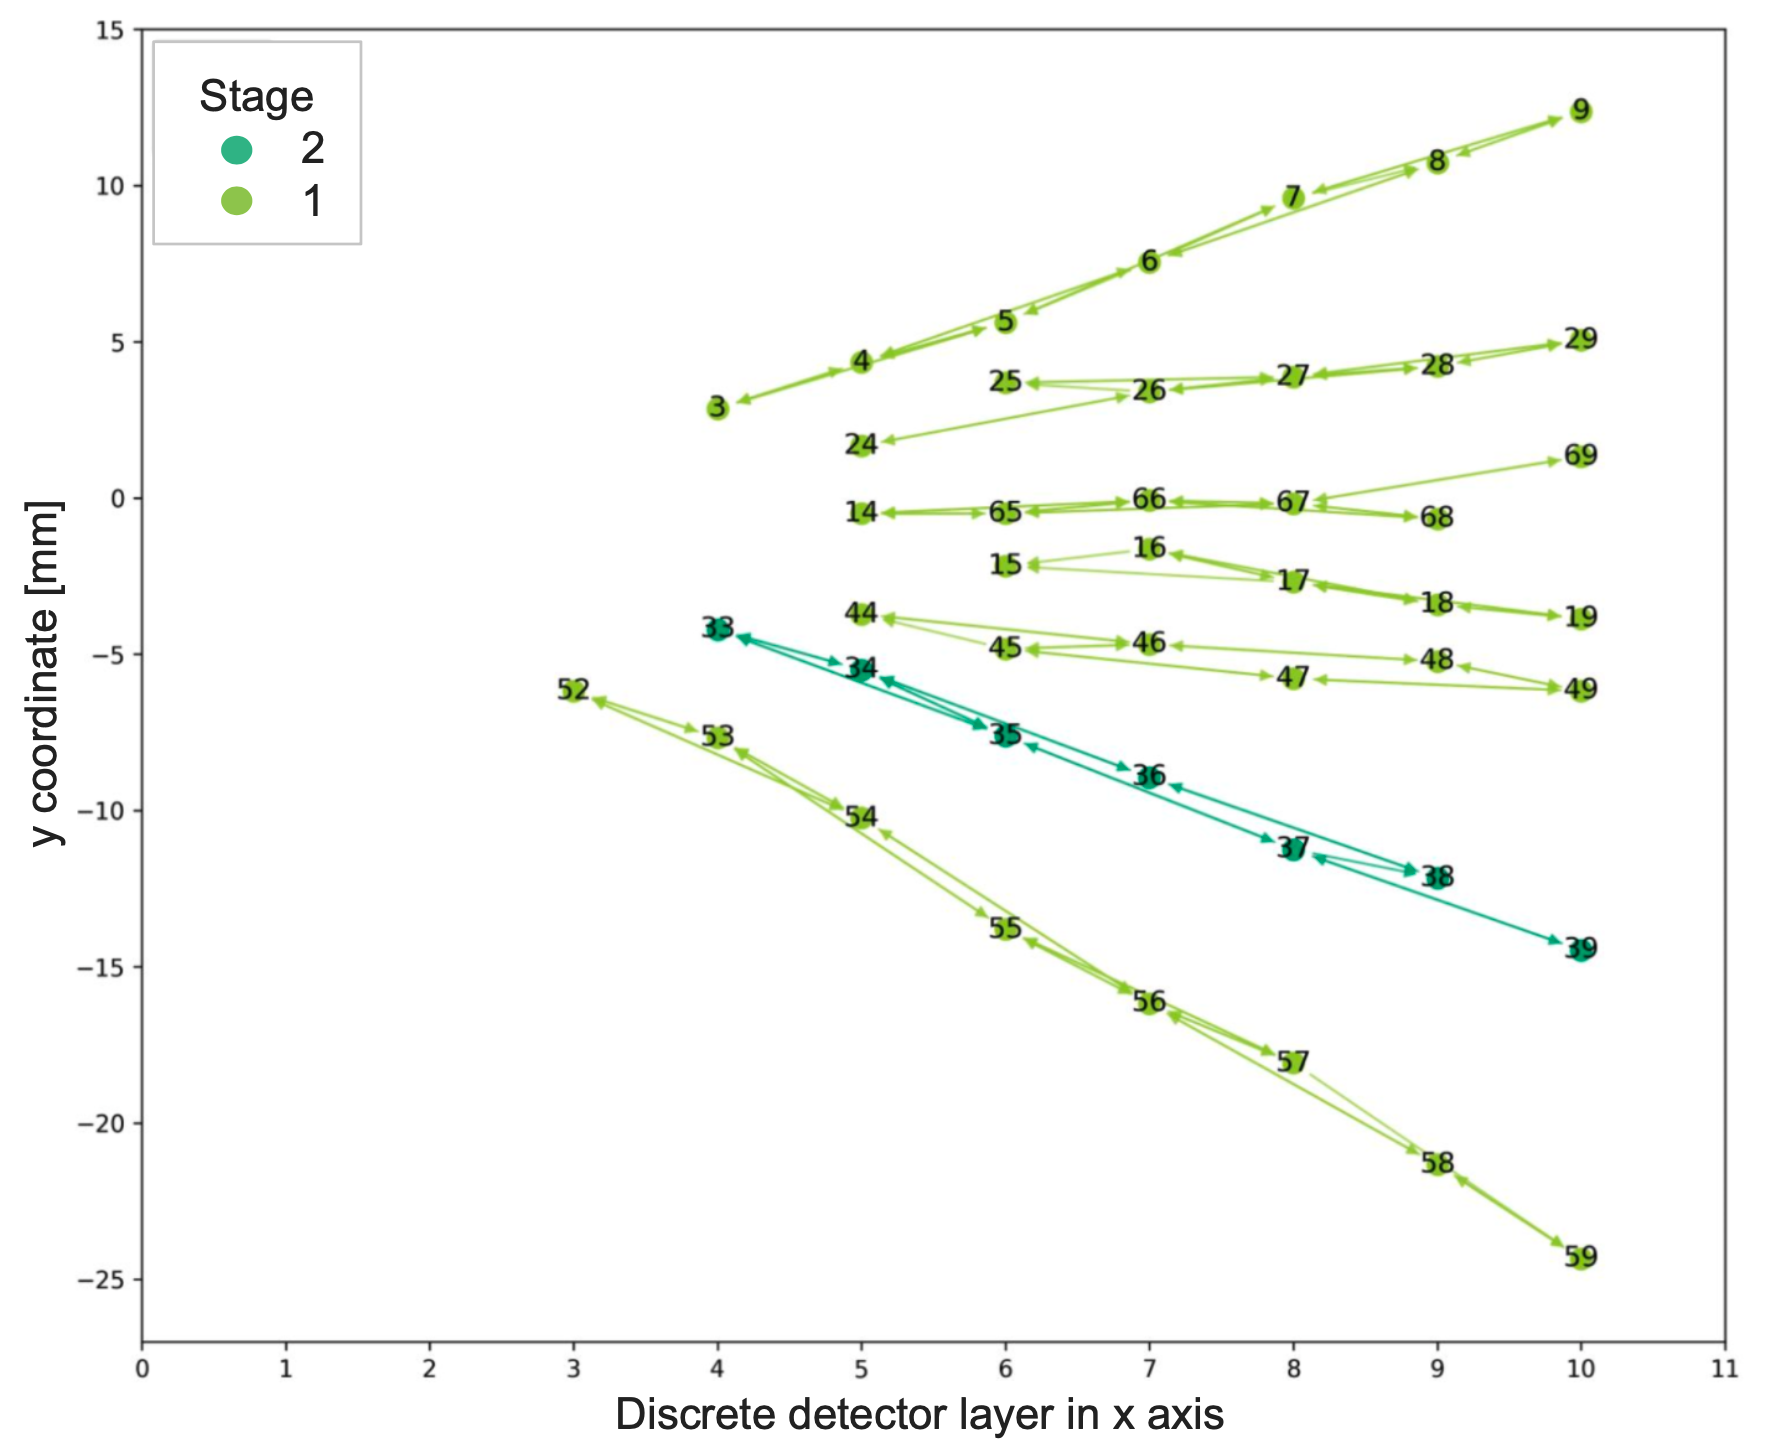
\includegraphics[width=12.1cm]{images/5-gnn-algorithm/mc-example-2a.png} } \label{fig:mc-example-2}}%
    \caption{Results of the GNN-based algorithm applied to a simple MC simulation. a) The simulated graph network where nodes with $\sigma_e^2 > 0.8$ are not plotted as clustering was not possible for these nodes. A CCA was applied to split the graph network into smaller subgraphs, where each colour indicates a different subgraph. b) The extracted track candidates after the applied GMR and Information Aggregation stages, where seven separate track candidates can be seen.}%
    \label{fig:example-application-1}%
\end{figure}
%\end{center}

%\begin{center}
\begin{figure}[htbp]%
    \centering
    \subfloat[\centering Simulated graph network post CCA]{{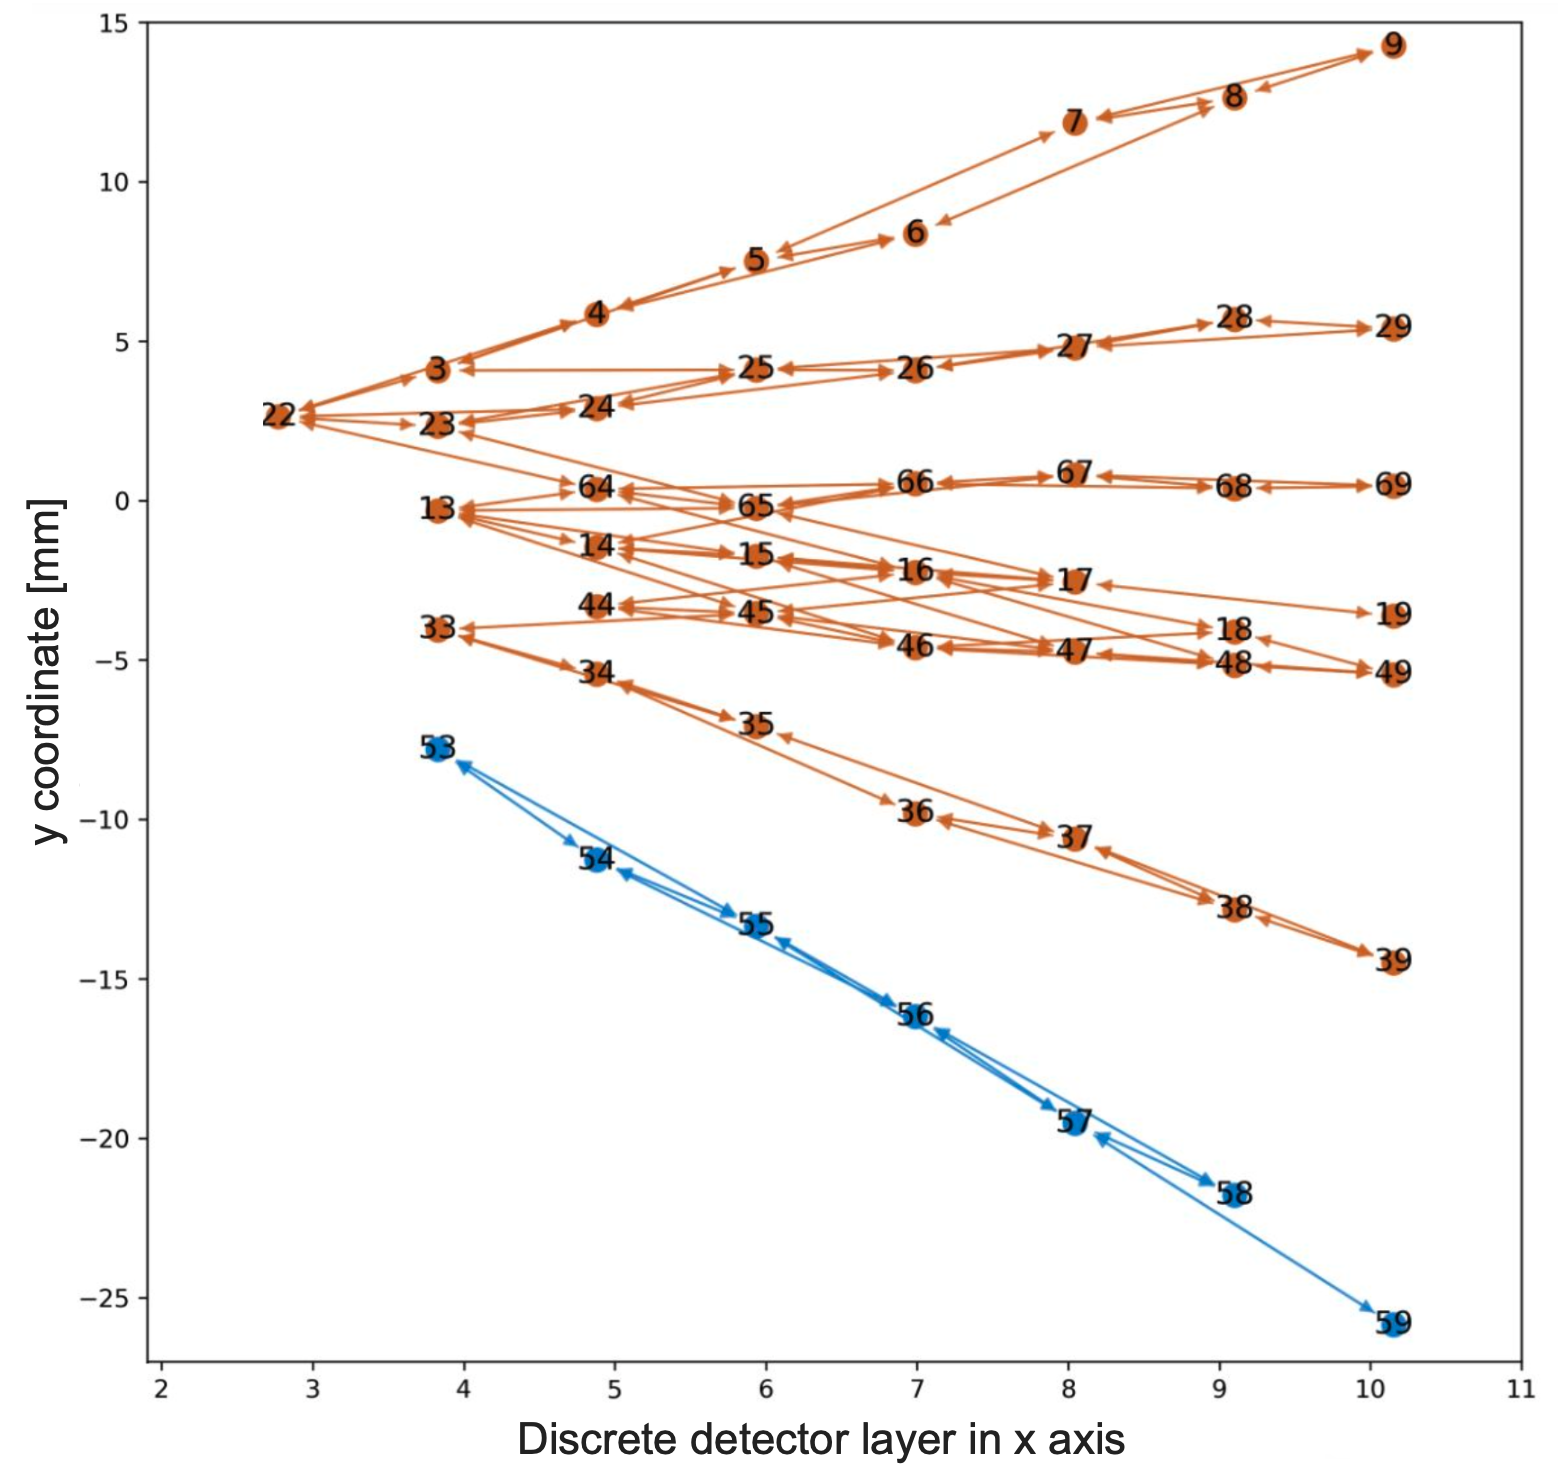
\includegraphics[width=10.7cm]{images/5-gnn-algorithm/mc-example-3a.png} } \label{fig:mc-example-3}}%
    \hfill
    %\qquad
    \subfloat[\centering Extracted track candidates after stage 1]{{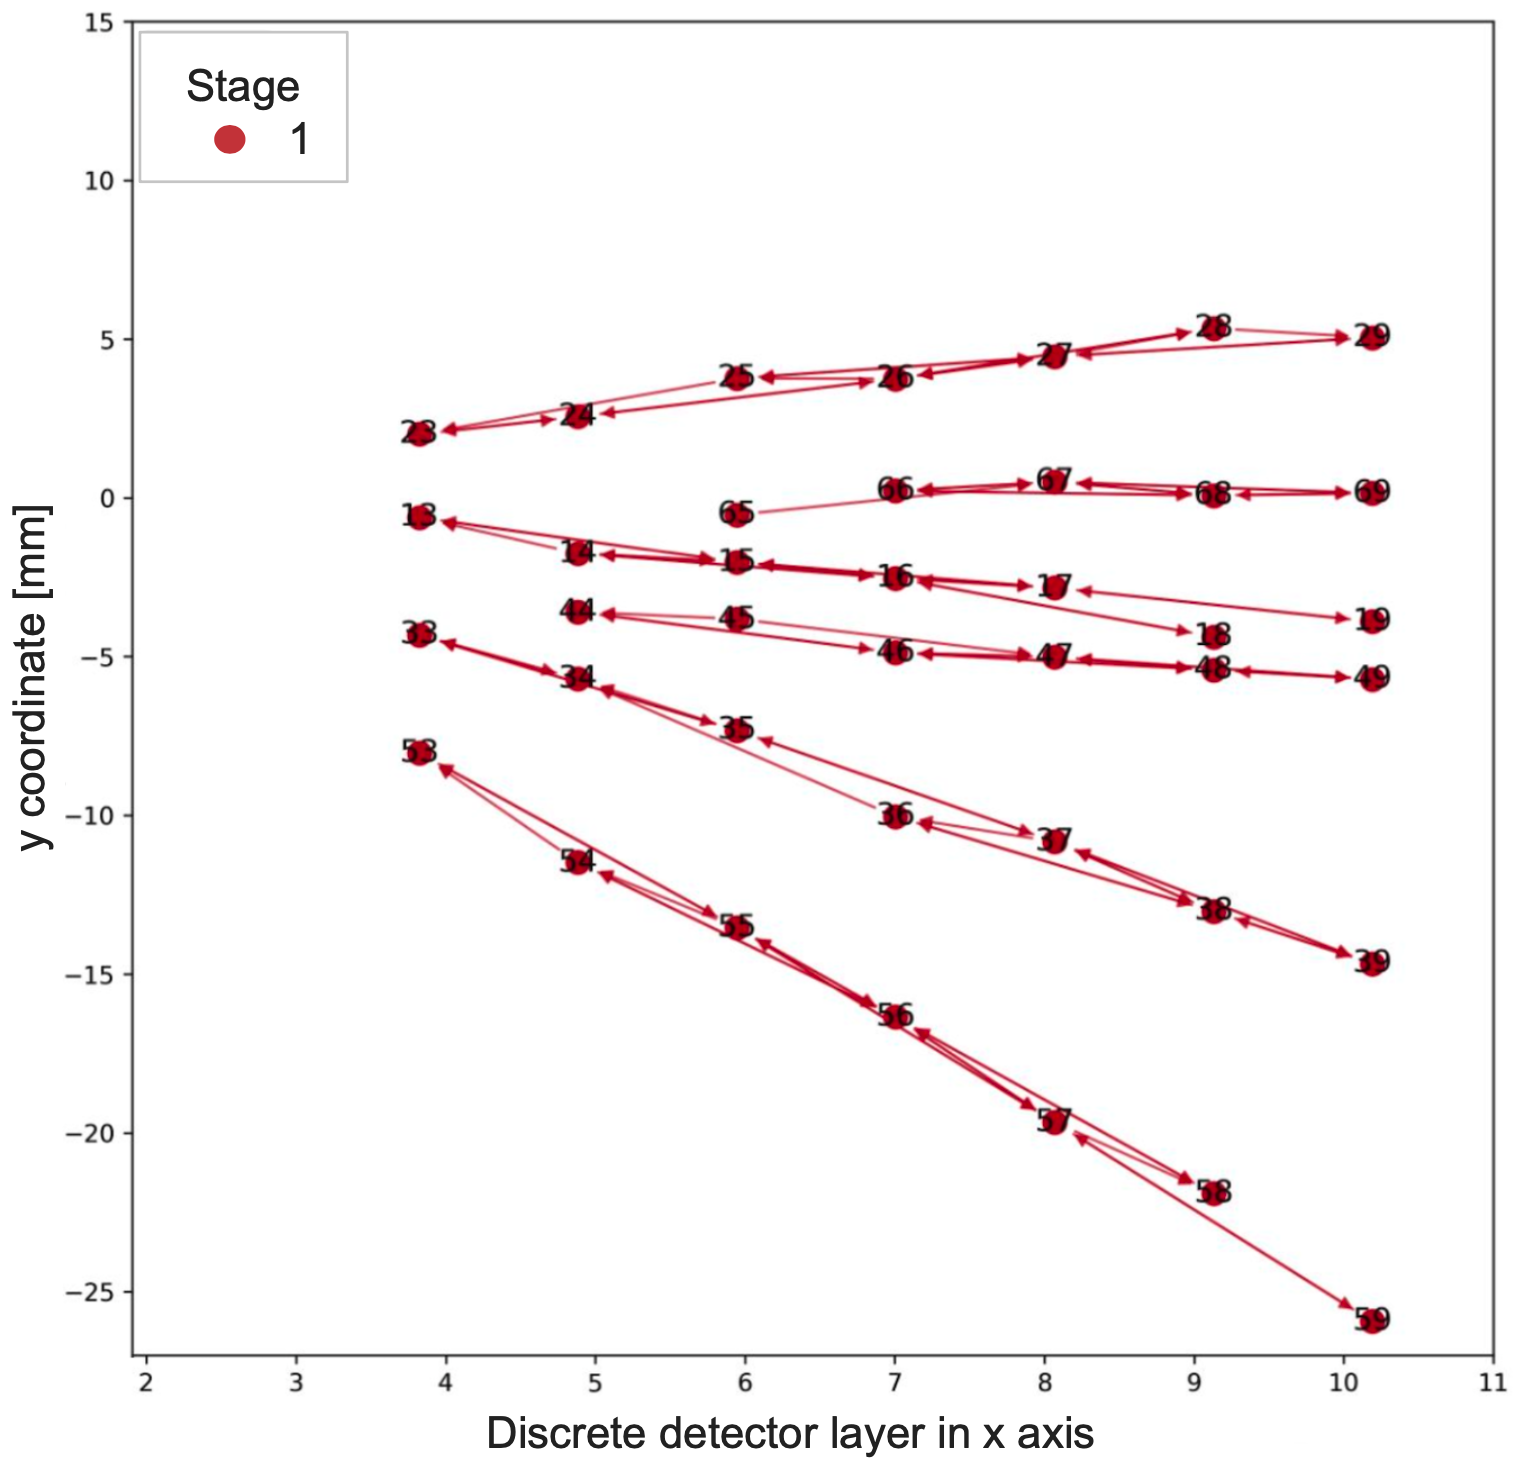
\includegraphics[width=10.8cm]{images/5-gnn-algorithm/mc-example-5a.png} } \label{fig:mc-example-4}}%
    \caption{Results of the GNN-based algorithm applied to a simple MC simulation a) The simulated graph network where nodes with $\sigma_e^2 > 0.8$ are not plotted as clustering was not possible. A CCA was applied to split the graph network into smaller subgraphs, where each colour indicates a different subgraph. b) Six extracted track candidates after the GMR stage.}%
    \label{fig:example-application-2}%
\end{figure}
%\end{center}


\section{Conclusion}

The proposed GNN algorithm is successful in iteratively identifying outlier edge connections and extracting track candidates for simple simulated particle collision events. GMR via clustering of state vectors proves to be a successful first step towards resolving incompatible connections in the network. The KF works well for both the extrapolation of state vectors to neighbour nodes, as well as for track extraction and track fitting. This ensures neighbourhood information can be aggregated in order to improve the precision in track state parameters. An intrinsic characteristic of the GNN algorithm is that neighbourhood complexity is inferred by the network. This is observed as the GNN algorithm automatically initiates the pattern recognition process in regions where outlier connections are easily identifiable. The network starts with low density regions and gradually progresses towards high density areas. This indicates that the GNN algorithm behaves as expected, first resolving ambiguities in ``cold'' regions and shows great promise for extraction of track candidates in more complex cases and realistic detector setups.


%It was observed that clustering of states was not always possible in all ``hot'' regions. As a result, the pattern recognition process was automatically initiated in regions where outlier connections were easily identifiable, i.e. ``cold'' regions. This indicates that the GNN algorithm behaves as expected, as the network starts with low density regions and gradually progresses towards high density areas.